\section{Results}
\label{sec:results}

\subsection{Evaluation Metrics}
\subsection{IoU Score}
Intersection over Union (IoU) is defined as the ratio of the area of intersection between the predicted segmentation map A and the ground truth map B to the area of their union.
\begin{equation*} 
\text{IoU}=  \frac{|A \cap B|}{|A \cup B|}. 
\end{equation*} 

\subsection{Quantitative Comparision}
% table
\begin{table}[h]
    \centering
    \begin{tabular}{|c|c|c|}
        \hline
        Model & mIoU(Val Set) & mIoU(Test Set) \\
        \hline
        UNet++ & 80.32 & 82.91 \\
        Graph-FCN & 83.94 & 83.45 \\
        CNNG & 82.93 & 84.33 \\
        MaskFormer & 88.85 & 86.11 \\
        Mask2Former & 88.70 & 86.16 \\
        TransUnet & 96.71 & 96.89 \\
        \hline
    \end{tabular}
    \caption{Comparison of mIoU scores on validation and test sets}
    \label{tab:results}
\end{table}

% table -> number of parameters
\begin{table}[h]
    \centering
    \begin{tabular}{|c|c|}
        \hline
        Model & Number of Parameters \\
        \hline
        UNet++ & \ 260.8M \\
        Graph-FCN & \ 609.91M \\
        CNNG & \ 609.92M \\
        TransUnet &  105.3M \\
        MaskFormer &  101.8M \\
        Mask2Former &  106.8M \\
        \hline
    \end{tabular}
    \caption{Comparison of number of parameters}
    \label{tab:results}
\end{table}

\subsection{Qualitative Comparision}
The qualitative comparison of segmentation results is shown in Figures \ref{fig:results} and \ref{fig:results2}.
% images
\begin{figure}[t]
    \centering
     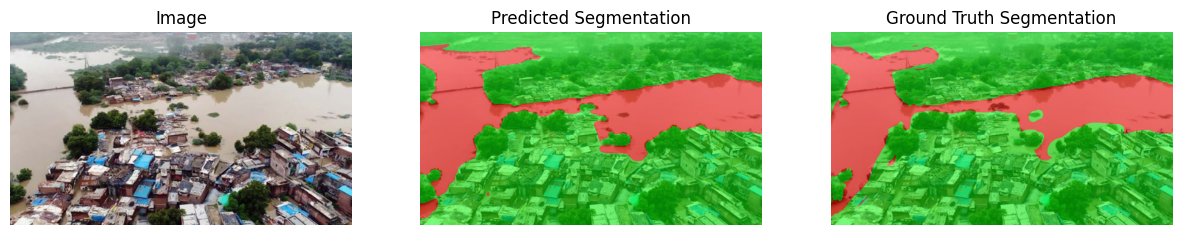
\includegraphics[width=0.9\linewidth]{images/maskformer_1_after.png}
  
     \caption{Qualitative comparison of segmentation results.}
     \label{fig:results}
\end{figure}

\begin{figure}[t]
    \centering
     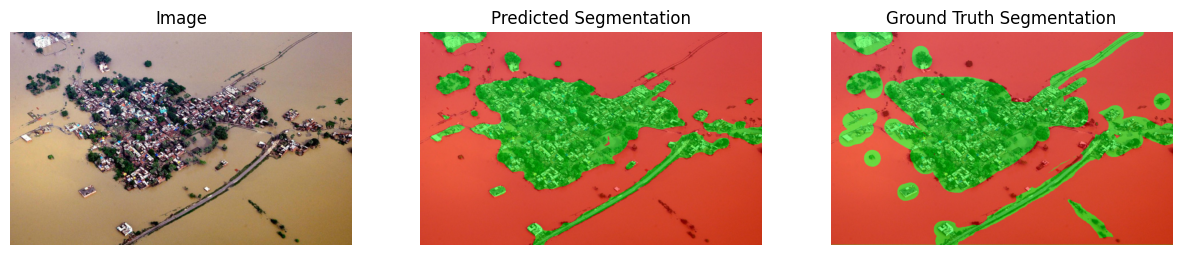
\includegraphics[width=0.9\linewidth]{images/maskformer_2_after.png}
  
     \caption{Qualitative comparison of segmentation results.}
     \label{fig:results2}
\end{figure}